\documentclass[nobib]{tufte-handout}
\usepackage[utf8]{inputenc}
\usepackage[estonian]{babel}
\usepackage[style=english]{csquotes}

\title{IDU1321 - Ettevõtte äriarhitektuur syllabus}
\author[Andres Kütt]{Andres Kütt}

%\date{04.08.2017}
%\geometry{showframe} % debug

\usepackage{natbib}

\usepackage{graphicx}
 \setkeys{Gin}{width=\linewidth,totalheight=\textheight,keepaspectratio}
  \graphicspath{{graphics/}} % set of paths to search for images
\usepackage{amsmath}  % extended mathematics
\usepackage{booktabs} % book-quality tables
\usepackage{units}    % non-stacked fractions and better unit spacing
\usepackage{multicol} % multiple column layout facilities
\usepackage{lipsum}   % filler text
\usepackage{fancyvrb} % extended verbatim environments
  \fvset{fontsize=\normalsize}% default font size for fancy-verbatim environments

% Standardize command font styles and environments
\newcommand{\doccmd}[1]{\texttt{\textbackslash#1}}% command name -- adds backslash automatically
\newcommand{\docopt}[1]{\ensuremath{\langle}\textrm{\textit{#1}}\ensuremath{\rangle}}% optional command argument
\newcommand{\docarg}[1]{\textrm{\textit{#1}}}% (required) command argument
\newcommand{\docenv}[1]{\textsf{#1}}% environment name
\newcommand{\docpkg}[1]{\texttt{#1}}% package name
\newcommand{\doccls}[1]{\texttt{#1}}% document class name
\newcommand{\docclsopt}[1]{\texttt{#1}}% document class option name
\newenvironment{docspec}{\begin{quote}\noindent}{\end{quote}}% command specification environment

\begin{document}
\maketitle
\begin{abstract}
\noindent
Käesolev dokument on Tallinna Tehnikaülikooli aine ``IDU1321 - Ettevõtte äriarhitektuur`` ainekaardi laiendus sisaldades bibliograafiat, igakordset lugemismaterjali ning praktikumi ülesandeid. Tegu on sisulisema lisandusega akadeemilisele ainekaardile, mis iganes lahkhelide korral kehtib ametlik ainekaart. Paber hakkab aine edenedes täienema, pea versioone silmas!
\end{abstract}

\section{Versioonid}
\begin{description}
	\item[4.0] Lisatud viienda loengu küsimused ja harjutuse näide
	\item[5.0] Kuuenda loengu sisu olemas
\end{description}

\section{Meetod}
Õpitulemused saavutatakse tuginedes järgmistele põhimõtetele
\begin{itemize}
	\item Teema on lai, seega kraabime vaid selle pinda vähestest, praktliselt kasulikest, kohtadest
	\item Valdkond on abstraktne, seega räägime samast asjast mitu korda eri nurkade alt. Pigem vähem aga sügavamat teadmist
	\item Eelistame akadeemilist teadmist raamistikele ja muule kommertsteabele. Esimene on püsiv väärtus, teised pigem mitte
	\item Modelleerimine on kommunikatsioonivahend, seega suhtume asjakohastesse standarditesse loovalt
	\item Tegemist on inseneeriaga, seega õpime tulemusi praktiliselt rakendama\sidenote{Kuna aega on vähe, vaatame ühte lähenemist paljudest. See konkreetne on valitud, sest tal on praktilised väljundid korporatiivkommunikatsioonis}
\end{itemize}

\section{Õpiväljundid}
Kursuse läbinud tudeng 
\begin{enumerate}
	\item Tunneb ettevõtte arhitektuuri ning äriarhitektuuri peamise mõisteid ja kontseptsioone, saab aru nende seosest infosüsteemidega 
	\item Oskab suurest süsteemist (nagu ettevõte ja tema infosüsteem) tervikpilti luua ja struktuurselt esitada. 
	\item Oskab struktuurselt mõelda ja arutleda. 
	\item Oskab modelleerida ettevõtte põhiprotsesse ning dekomponeerida neid kasutuslugudeks, funktsionaalseteks komponentideks ja tehnoloogilisteks lahendusteks
	\item Tunneb ja oskab kasutada vähemalt ühte infosüsteemi strateegilise analüüsi ja ärimodelleerimise metoodikat. 
	\item Oskab kasutada UMLi ja ORMi strateegilise analüüsi põhimudelite ja -vaadete koostamiseks 
	\item Oskab täita äriarhitekti, ärianalüütiku ja äridisaineri rolle infosüsteemi strateegilise analüüsi projektides. 
	\item Teab keerukuse ja selle juhtimise põhimõisteid
	\item Oskab eri vaatepunktidest hinnata lihtsamate süsteemide keerukust
	\item Oskab luua ja analüüsida seoseid organisatsiooni, selle strateegia ning infosüsteemi vahel
\end{enumerate}

\section{Loengud/praktikumid}
Aine sisu on toodud tabelis \ref{tab:content}. Loengus ja praktikumis osalemise eelduseks on, et viidatud artiklid, ja presentatsioonid on läbi loetud\sidenote{Raamatute läbimist ei eelda, need on toodud teemaga süvitsi minna soovijatele}. Loengu eesmärk on loetut täiendada, vastata küsimustele ning siduda eri allikaid. Kirjandust loengus ümber ei jutustata, edukas eksam eeldab sellega tutvumist. 

Loeng koosneb kolmest osast:
\begin{enumerate}
	\item Käime üle peamised ideed, mõisted ja kontseptsioonid
	\item Tegeleme kas kõik koos või väiksemates rühmades harjutustega
	\item Kokkuvõte harjutustest, sissejuhatus järgmisse teemasse ja ülevaade kirjandusest
\end{enumerate}

\renewcommand{\arraystretch}{1.3}
\begin{table*}[ht]
\small
	\centering
	\fontfamily{ppl}\selectfont
	\begin{tabular}{lp{5cm}p{6cm}p{4cm}}
		\toprule
		& Loeng & Harjutus & Kirjandus\\
		\midrule
		1 & Aine struktuur ja akadeemiline kontekst. EA ja ümberkaudsed mõisted. Ettevõttearhitekti roll. Eri vaated ettevõttele & Mida teeb ettevõttearhitekt Microsoftis, Eesti Energias, Swedpankis, Riigi Infosüsteemi Ametis, Transferwise's?  & \cite{parsons2005enterprise}; \cite{hickey}; \cite{sysengineering}; \cite{winter2006essential}\\
		2 & Modelleerimine. Kasud, kahjud. UMLi ja ORMi põhitõed. Staatilised ja dünaamilised vaated. & Modelleerime: Kohvitass, ERP & \cite{OPM}; \cite{heumann2005introduction}, \cite{box1976science}, \cite[peatükk 3]{ferenvcik2004survey}\\
		3 & Arhitektuur, väärtus ja äri. Strateegia ja arhitektuur & Lahkame organisatsiooni: EMTA & \cite{gadiesh2001transforming}; \cite{senge2002leader}\\
		4 & Äriprotsess ja kasutuslood & Modelleerime maksekorralduse protsessi & \cite{checkland2000soft} esimene pool \\
		5 & Äriprotsessist infosüsteemini. Linnaplaneerimine & Maksekorralduse jäljed süsteemis & \cite{wohed2006suitability}; \cite{bertin2014urbanization}\\
		6 & Infosüsteemist äriprotsessini. Infosüsteemi mõju organisatsioonile. Conway seadus, selle implikatsioonid & Tegeleme demokraatliku innovatsiooni tagajärgedega & \cite{conway1968committees}; \cite{maccormack2012exploring}\\
		7 & Süsteemiarhitektuuri alused & & \cite{crawley2015system}\\
		8 & Keerukus ja selle juhtimine & & \cite{holt2017so}\\
		\bottomrule
	\end{tabular}
	\caption{Loengute teemad, ülesanded ja kirjandus}
	\label{tab:content}
\end{table*}

\section{Iseseisev töö}
Ainekaardilt: \enquote{Ülesandeks on välja töötada konkreetse (reaalse või väljamõeldud) organisatsiooni infosüsteemi viiekihiline mudel. Lähtudes konkreetsest äriprotsessist koostatakse organisatsiooni, kasutuslugude, funktsionaalsete osiste ja tehniliste komponentide mudelid. Tulemus kantakse ette.}

\section{Loengud}
\subsection{Esimene}

Kordamisküsimused kirjanduse tarbeks on järgmised:
\begin{itemize}
	\item Mis on ettevõttearhitekti\sidenote{Parema puudumisel kasutame siin ja edaspidi toortõlget ingliskeelsest \emph{Enterprise Architect}i mõistest} roll \citeauthor{parsons2005enterprise}, \citeauthor{sysengineering} ja \citeauthor{winter2006essential} arvates, mis on peamised erinevused?
	\item Mis on peamised EA kihid \cite{winter2006essential} järgi?
	\item Millistest kuus vaadet eksisterivad arhitektuurile \citeauthor{sysengineering} järgi? Millisesse neist kuuluvad ORM ja UML?
	\item Mis on \citeauthor{hickey} järgi peamine EA probleem agiilses transformatsioonis ning mis on peamised viisid selle ületamiseks?
\end{itemize}

Harjutuseks arutame koos ettevõttearhitekti rolli üle eri tüüpi ettevõtetes. Rolli põhiküsimused on:
\begin{itemize}
	\item Mis on lahendatav põhiprobleem?
	\item Kellele raporteeritakse?\sidenote{Laiemalt, kus organisatsioonis roll paikneb. Pane tähele, kuidas roll sõltub organisatsiooni struktuurist}
	\item Millised on õigused ja kohustused?
	\item Mis on kontrollitava süsteemi ulatus?
	\item Kes on otsesed ja kaudsed alluvad?
\end{itemize}

Vaadeldavad organisatsioonid:
\begin{itemize}
	\item Microsoft kui hiiglaslik rahvusvaheline tarkvaraettevõte
	\item Eesti Energia kui suur tehnoloogiaettevõte
	\item Swedbank Baltic kui rahvusvaheline osa suurest rahvusvahelisest mitte-tehnoloogiaettevõttest
	\item Riigi Infosüsteemi Amet kui taristut pakkuv riigiasutus
	\item Transferwise kui kasvufaasi iduettevõte\sidenote{Pane tähele, kuidas tegu on hübriidiga finants- ja tehnoloogiaettevõttest}
\end{itemize}

\subsection{Teine}
Kordamisküsimused kirjanduse tarbeks on järgmised:
\begin{itemize}
	\item Mis on põhimõtteline vahe UML ja ORM mudelite vahel?
	\item Mis elemendid on kaasatud igasse kommunikatsiooni?
	\item Kuidas suhtub mudel füüsilisse reaalsusse?
\end{itemize}

Modelleerime kohvitassi ja ERP\sidenote{\emph{Enterprise Resource Planning}} süsteemi. Mõlema puhul esitame küsimused:
\begin{itemize}
	\item Miks me modelleerimie?
	\item Mida \emph{kasulikku} see asi teeb?
	\item Millistest tükkidest ta koosneb?
	\item Millised on seosed tükkide ja funktsiooni vahel?
\end{itemize}

\subsection{Kolmas}
Kordamisküsimused kirjanduse tarbeks on järgmised:
\begin{itemize}
	\item Mis on strateegilise printsiibi peamised omadused?
	\item Mis on loominguline pinge ja kuidas ta tekib?
	\item Millised on Senge järgi liidri rollid õppivas organisatsioonis?
\end{itemize}

Uurime, EMTA arhitektuuri vastates ettevõtte arhitekti positsioonilt küsimustele
\begin{itemize}
	\item Mida EMTA teeb?
	\begin{itemize}
		\item Kellele luuakse väärtust?
		\item Läbi milliste tegevuste?
	\end{itemize}
	\item Kuidas EMTAst mõelda?
	\begin{itemize}
		\item Kust tuleneb EMTA strateegia?
		\item Millises juriidilises kontekstis ta tegutseb?
		\item Milline võiks olla EMTA kultuur?
	\end{itemize}
	\item Millest EMTA koosneb?
	\begin{itemize}
		\item Millised on peamised organisatsioonilised üksused\sidenote{\url{www.emta.ee} on abiks}?
		\item Mis peamisi infosüsteeme EMTA kasutab?
		\item Milline on organisatsiooni füüsiline kontekst?
	\end{itemize}
\end{itemize}

\subsection{Neljas}
Kordamisküsimused kirjanduse jaoks
\begin{itemize}
	\item Milles erinevad \enquote{pehme} ja \enquote{kõva} suhtumine süsteemidesse?
	\item Kuidas kirjeldada tegevust PQR mudeli järgi?
	\item Millistest loogilistest sammudest koosneb tegevusmudeli koostamine?
\end{itemize}

\subsection{Viies}
Kordamisküsimused kirjanduse jaoks
\begin{itemize}
	\item Miks ja mis faasides suurte süsteemide struktuur arenduse käigus laguneb?
	\item Miks ei ole mõistlik konteksti lisamata rääkida süsteemi ühest konkreetsest disainist?
\end{itemize}

\begin{figure}%
\begin{center}
  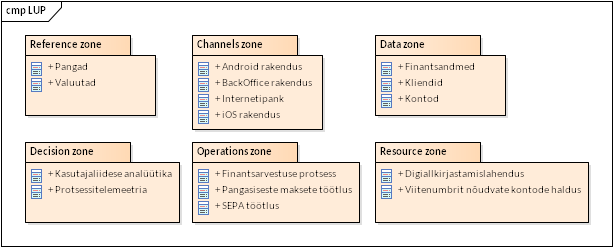
\includegraphics[width=\linewidth]{harjutus_lup}
  \caption{Harjutuse käigus koostatud LUP, üks paljudest võimalikest}
  \label{fig:harjutus}
\end{center}
\end{figure}

\subsection{Kuues}
\newthought{Ühes suures tehases töötas hr. Starostin.} Tehas oli suur ja kuulus veel suuremasse kontserni, kus sedalaadi käitiseid oli palju. Ei ole tähtis, mis ametit Starostin seal tehases pidas. Oluline on vaid, et ta suhtles tehase Tähtsa Direktoriga igapäevaselt. Tähtis Direktor pidi igakuiselt raporteerima oma ülemustele kõikvõimalikke numbreid tehase toimimise kohta. Sealhulgas erinevaid parameetreid heitmete --- $CO_2$, heitveed ja nende koostis, jne. --- kohta. Nii oli alati olnud. Insenerid lugesid oma ringkäikudel seierite näidud, kirjutasid need üles ning sekretär vormistas neist Tähtsa Direktori jaoks aruande. See kõik oli tüütu, sest inseneridel oli muudki teha, kui paberitega ringi joosta ja sekretär ajas alailma kilomeetrid kilogrammidega segi. 

\newthought{Aga hr. Starostin oli kooli ajal veebilehtesid teinud.} Ta teadis, et tehas oli küllalt moodne ning tegelikult olid kõigi nonde seierite taga digitaalsed andurid. Ja tal sündis plaan. Ta hankis peainsenerilt vajaliku dokumentatsiooni ning pusis nädalavahetusega kokku rakenduse, mis igal ööl anduritega ühendust võttis ning andmed baasi kirjutas. Aga baasi otsa ehitas ta lihtsa veebilehe, mis sealt andmed võttis, kokku liitis ning aruande vormiks kujundas. Kõik olid õnnelikud: sekretäri pea ei valutanud enam, insenerid said oma tööd teha ja Tähtis Direktor ei jäänud enam ülemuste ees lolliks. Starostin sai kiita. Tähtis Direktor sai aru, et seda inimest ära kasutades sai ta suure hulga tehase igapäevase opereerimise tüütutest probleemidest lahendada ilma, et oleks pidanud keskse it-organisatsiooni tüütute protsessidega jandama. Või nende arveid maksma. Isegi keskne it-organisatsioon oli rahul, sest nad said tegeleda Oluliste Asjadega selle asemel, et mingi tehase pisiasjadele mõelda. Pealegi oli siin tegemist ebameeldivalt keeruliste SCADA süsteemidega mille torkimiseks piisava pikkusega pulka ei olnud peakontori tarkvarainseneride meelest veel välja mõeldud. 

\newthought{Ja siis tekkis EU kasvuhoonegaaside turg.} tehase korstnast välja paiskuv heide oli ühtäkki väärtuslik. Ja võime seda mõistlikult juhtida rangelt jälgitud. Kontserni it-organisatsioon sai ülesande korraldada kontserniülene $CO_2$ ja muude heitmete andmete kogumine ja mitmes eri väljundis raporteerimine. Hr. Starostini aastate jooksul kokku kirjutatud skriptid muutusid üleöö ärikriitiliseks. Olemata samas selleks üldse võimelised: Starostini vene-, eesti- ja inglise segakeeles muutujanimedega kommenteerimata ja failinimede abil versioneeritud klasterdamata MySQL lahendus oli väga kaugel tavapärasest arusaamast kõrgkäideldavast ärikriitilisest lahendusest. Kuid ta jätkas kangekaelselt toimimist. Ja Tähtis Direktor keeldus sama kangekaelselt oma kuludesse võtmast uut ja kallist andmekogumisrakendust. 



\section{Lisalugemist}
\begin{itemize}
	\item Üldist
	\begin{itemize}	
		\item \cite{simon1996sciences}. Huvitav ja suhteliselt populaarne käsitlus keerulistest süsteemidest 
		\item \cite{stanford2005guide}.Economisti põhjalik vaade organisatsiooni kui sellise disaini
		\item \cite{checkland2000soft}. Väga hea (kuigi pikk) käsitlus süsteemiteooria rakendamiest ärilises kontekstis. Sisaldab väga korralikku bibliograafiat
	\end{itemize}
	\item UML
	\begin{itemize}
		\item \cite{fatolahi2006investigation}. Üsna põhjalik käsitlus Zachmani EA raamistikust ja selle rakendamisest UMLi abil. Hulgaliselt kasulikke viiteid, päris hea sissevaade akadeemilisse modelleerimsie ja EA maailma
		\item \cite{umldistilled} Hästi käepärane maakeelne UMLi käsiraamat
	\end{itemize}
	\item Kommunikatsioon ja modelleerimine
	\begin{itemize}
		\item \cite{shannon2001mathematical}. Kommunikatsiooniteooria tüvitekst. Esimene koht, kus räägitakse kommunikatsiooniprotsessi elementidest
		\item \cite{tufte}. Kohustuslik kirjandus igaühele, kes edastab keerulise struktuuriga kvantitatiivset informatsiooni
	\end{itemize}
	\item Organisatsioonid
	\begin{itemize}
		\item \cite{cohen2007influence}. Kuidas ilma formaalse võimuta asju tehtud saada? \cite{cohen1989influence} on samade autorite varasaem artikkel samal teemal\sidenote{Ei ole avalikult kättesaadav}
		\item \cite{senge2006fifth}. Pikem, raamatu formaadis, versioon kohustuslikust lugemisest \cite{senge2002leader}. Väga väärt ja potentsiaalselt maailmapilti muutev lähenemine õppivale organisatsioonile\sidenote[][-10mm]{Õppiv organisatsioon kui idee on viimase kümnendiga arenenud edasi dünaamiliste võimekuste teooriaks, see läheb aga meie teemast liiga kaugele}
		\item \cite{optner}. Kui kellelegi pakuvad huvi\sidenote{Ja kui keegi kätte saab. Euroopast koopiat ei leidnud, Stanfordi raamatukogus üks oli. Viide \cite{checkland2000soft} kaudu} süsteemse organisatsioonikäsitluse juured
		\item \cite{freedman2013strategy}. Suurepärane (kuid mahukas) Lääne strateegiamõtte ajalugu koos kõigi olulisemate mõttevoolude, nimede ja publikatsioonidega. \sidenote{Freedmani video-loengud on kindlasti väärt vaatamist. Näiteks \url{https://www.youtube.com/watch?v=-R7kjNT8hkI}}
	\end{itemize}
	\item Arhitektuur
	\begin{itemize}
		\item \cite{longepe2003enterprise}. Huvitav, peamiselt frankofiilses kultuuriruumis, levinud käsitlus ettevõtte arhitektuurist ning selle paralleelidest linnaplaneerimisega
	\end{itemize}
\end{itemize}

\bibliography{idu1321}
\bibliographystyle{plainnat}
\end{document}